% Instructions to change to html version:
% Comment out:
%  minipage, multicols,columnbreak, mathbf, hrule
% Replace all: \begin{minipage}% \end{minipage} %\begin{multicols}  %\end{multicols}  %\columnbreak %% \begin{framed} %\end{framed} %%\hrule
% Replace \mathbf with \boldsymbol
% Replace $$ with \[ and $ with \(
% Enclose graphics in figure environments and add captions
% 			search \includegraphics
% Re-tag \df environments as sections, subsections, etc.
% Command Line Code to Create html version:
%First: pdflatex -shell-escape filename.tex                                   
%Second, for each figure: inkscape "filename-figure1.pdf" -o "filename-figure1.png"
% Third: htlatex filename.tex "ht5mjlatex.cfg, charset=utf-8" " -cunihtf -utf8"

\documentclass[10pt]{article}

%\usepackage{tikz, pgf,pgfplots,wasysym,array}
%\usepackage{wasysym,array}

\usepackage{amsmath,amssymb}

\ifdefined\HCode
  \def\pgfsysdriver{pgfsys-tex4ht-updated.def}
\fi 
%\ifdefined\HCode
%  \def\pgfsysdriver{pgfsys-dvisvgm4ht.def}
%\fi 
\usepackage{tikz}
\usetikzlibrary{calc,decorations.markings,arrows}
\usepackage{pgfplots}

\pgfplotsset{compat=1.12}
\usepackage{myexternalize}
\usetikzlibrary{calc,decorations.markings,arrows}
\usepackage{framed}
\usepackage[none]{hyphenat}

\input{../../../common/1336_header_test.tex}
\begin{document}

\everymath{\displaystyle}


\newcommand{\ihat}{\boldsymbol{\hat{\textbf{\i}}}}
\newcommand{\jhat}{\boldsymbol{\hat{\textbf{\j}}}}
\newcommand{\khat}{\boldsymbol{\hat{\textbf{k}}}}

\let\oldvec\vec
\renewcommand{\vec}[1]{\oldvec{\boldsymbol{#1}}}

\renewcommand{\u}{\vec{u}}
\renewcommand{\v}{\vec{v}}
\newcommand{\w}{\vec{w}}
\renewcommand{\r}{\vec{r}}
\renewcommand{\a}{\vec{a}}
\renewcommand{\b}{\vec{b}}
\renewcommand{\c}{\vec{c}}

\newcommand{\<}{\left\langle}
\renewcommand{\>}{\right\rangle}

\renewcommand{\myTitle}{MATH 1336: Calculus III}

\renewcommand{\mySubTitle}{Section 2.3: The Dot Product}%\\
%Section 2.2: Vectors Group Work}
%~\hfill Name: \underline{~~~~~~~~~~~~~~~~~~~~~~~~~~~~~~~~~~~~~~~~~~~~~~~}
\lectTitle{\vspace*{-.5in}\myTitle}{\vspace*{.1in}\mySubTitle \vspace*{-.25in}}


\setlength{\columnseprule}{0.4pt}
\setlength{\columnsep}{3em}

%\hspace*{-.8in}%\begin{minipage}{1.25\textwidth}
%\begin{framed}

\section*{Intro to the Dot Product:}




%\begin{minipage}{.4\textwidth}


\begin{figure}[!h]
\centering
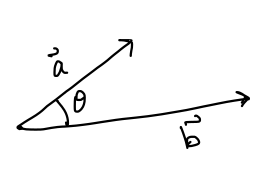
\includegraphics[height=1in]{dot-product.png}
\caption{Diagram showing two vectors and the angle between them.}
\end{figure}

%\vspace*{1in}
%
%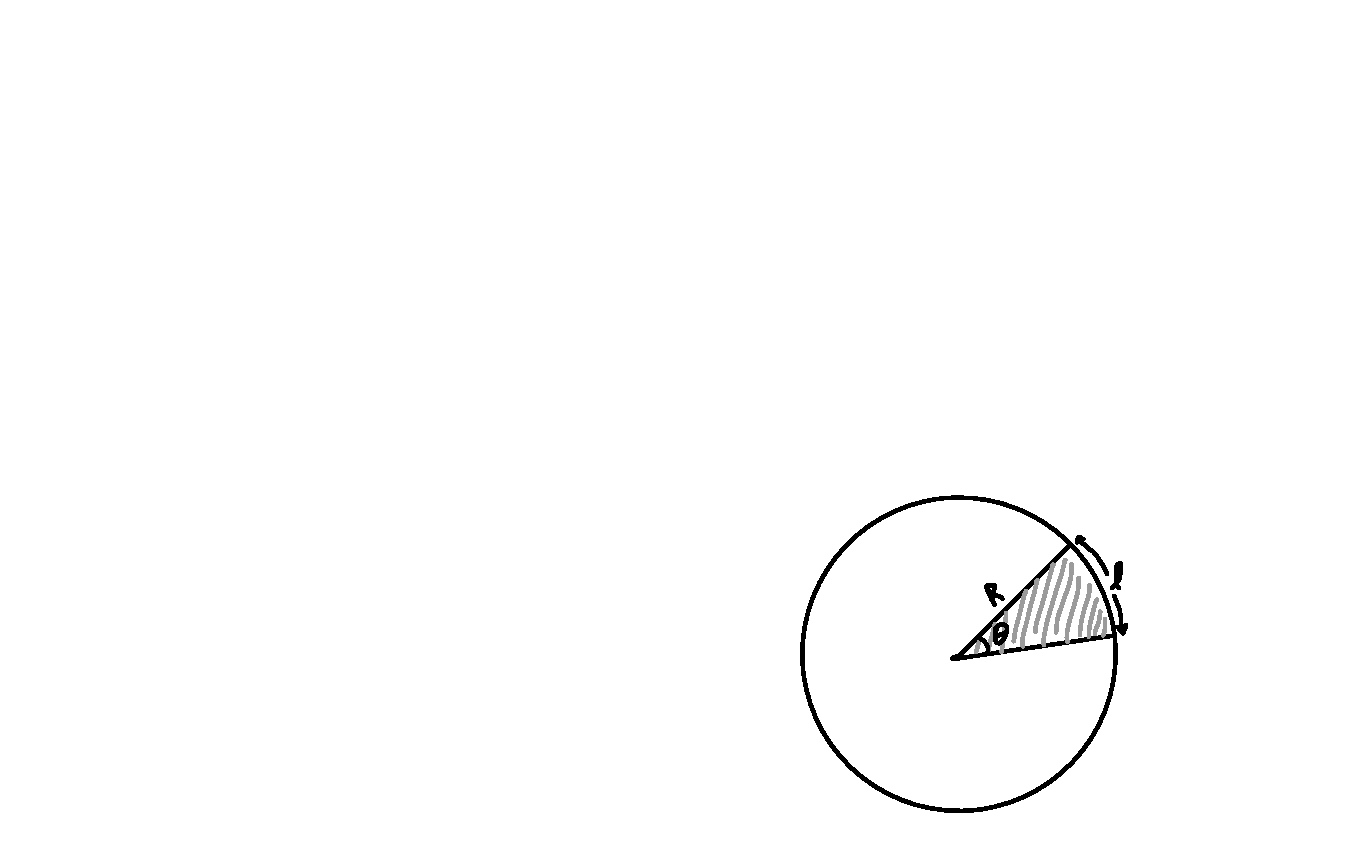
\includegraphics[height=1.5in]{circular-sector}


%\end{minipage}
\hspace*{.2in}
%\begin{minipage}{.5\textwidth}

%\textbf{Vocabulary \& Definitions:} \\~\\
The \textbf{dot product} of two vectors, \(\vec{a}=\<a_1,a_2,a_3\>, \b=\<b_1,b_2,b_3\>\) can be calculated using either formula below, where \(\theta\) is the angle between the two vectors\\
\[\a \cdot \b = a_1 b_1 + a_2 b_2 + a_3 b_3, \qquad \vec{a} \cdot \vec{b} =| |\a||\  ||\b||\ \cos \theta\]



%\vspace*{-.2in}
%\end{minipage}

%\end{framed}
%\end{minipage}

\section*{Examples:}
Calculate the following quantities, or explain why they don't make sense:

%\begin{mulitcols}{2}
\begin{enumerate}[{Example} 1.\(\quad\)]

\item \(\< 1, 2, 3\> \cdot \<4, 5, 6\>\)
\vspace*{.5in}

\item \(\< 1,-2\> \cdot \<-1, 2\>\)
\vspace*{.5in}

\item \(\< 0,1\> \cdot \<1,0\>\)
\vspace*{.5in}

\item \(\< 1,2\> \cdot \<1, 2\>\)
\vspace*{.5in}

\item \(\< 0,1, 2\> \cdot \<3, 4\>\)
\vspace*{.5in}

\end{enumerate}
%\end{multicols}

\section*{Discussion:}
Geometric Implications of  \(\vec{a} \cdot \vec{b} =\vec{a} \cdot \vec{b} =| |\a||\  ||\b||\ \cos \theta\)


%\pagebreak

%\section*{Group Work from the Textbook:}
%
%\vspace*{-.25in}
%\includegraphics[width=\textwidth]{Ch10s2_Group_Work.pdf}

%\hspace*{-.8in}%\begin{minipage}{1.25\textwidth}
%\begin{framed}


\subsection*{Properties of the Dot Product:}
\vspace*{-.2in}
%\begin{mulitcols}{2}
%The \textbf{dot product} of two vectors, \(\vec{a}=\<a_1,a_2,a_3\>\),\\
%\( \b=\<b_1,b_2,b_3\>\) can be calculated using either formula below, where \(\theta\) is the angle between the two vectors\\
%\[\a \cdot \b = a_1 b_1 + a_2 b_2 + a_3 b_3, \qquad \vec{a} \cdot \vec{b} = |\a| |\b| \cos \theta\]

~\\~\\
Two vectors are \textbf{orthogonal} (perpendicular) if-and-only-if \(\a \cdot \b = 0\).\\~\\

%\columnbreak

\(\u, \v, \w\) are all vectors in either \(\mathbb{R}^2\) or \(\mathbb{R}^3\), and \(c\) is a scalar 
\begin{enumerate}
\item \(\u \cdot \v = \v \cdot \u\)
\item \(\u \cdot \left(\v +\w\right) = \u \cdot \v + \u \cdot \w\)
\item\( c(\u \cdot \v) = (c\u)\cdot \v  = \u \cdot (c\v)\)
\item \(\v \cdot \v = ||\v||^2\)
\item \(\vec{0} \cdot \u = 0\)
\end{enumerate}

%\end{multicols}

%\hrule
\vspace*{.1in}

\subsection*{Projections:}
\underline{Definition:} The \textbf{vector projection} of \(\v\) onto \(\w\) is the vector labeled \(\u\) on the diagram shown below.\\
 It has the same initial point as \(\v\) and \(\w\), and represents the component of the vector \(\v\) that acts in the direction of \(\w\).\\
 The length of this vector is called the \textbf{scalar projection} of \(\v\) onto \(\w\).\\


%\begin{minipage}{.4\textwidth}


\begin{figure}
\centering
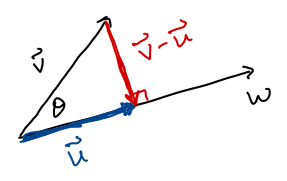
\includegraphics[height=1in]{Ch10s3-projections.png}
\caption{Diagram illustrating the projection of vector v onto vector w.}
\end{figure}

%\vspace*{1in}
%
%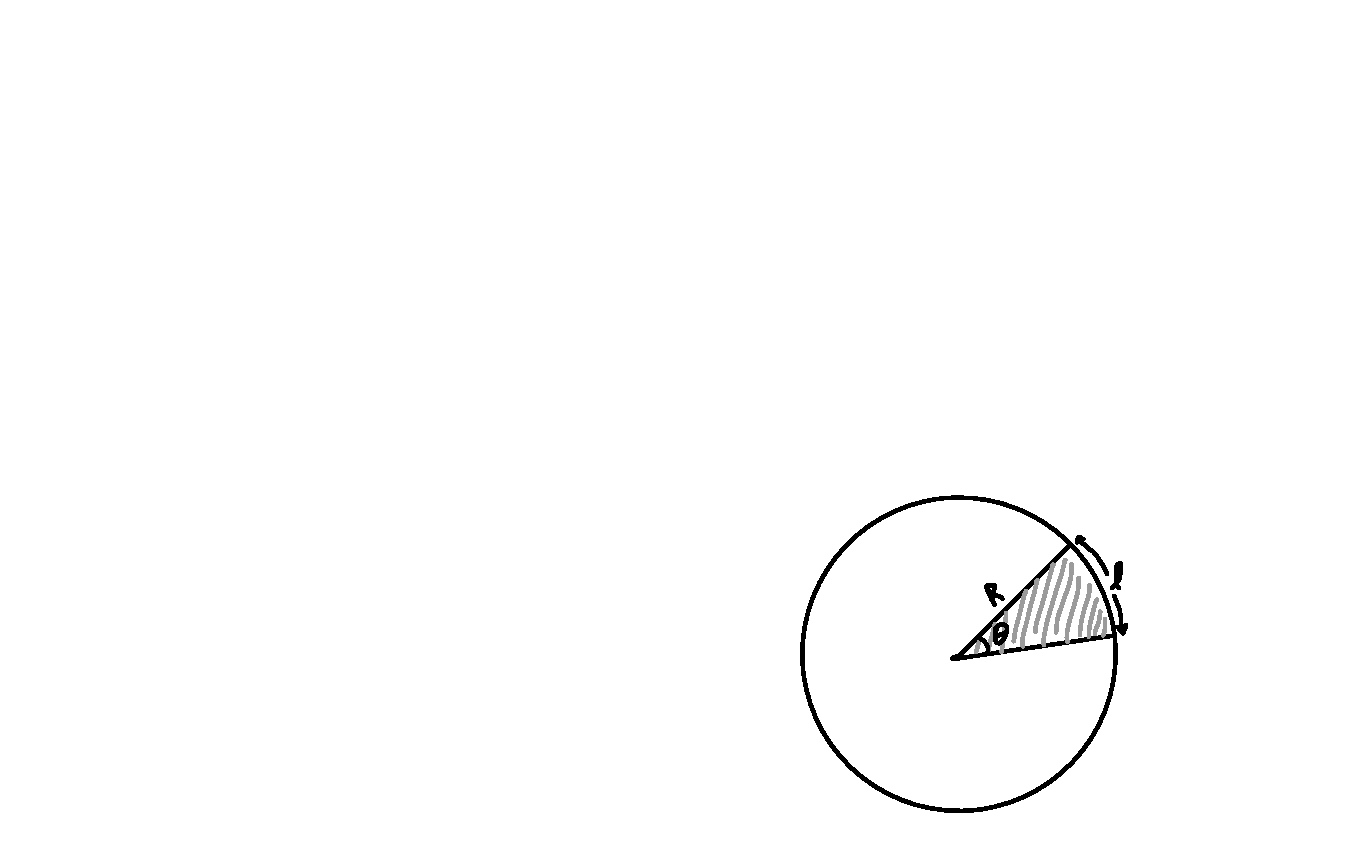
\includegraphics[height=1.5in]{circular-sector}


%\end{minipage}
\hspace*{.2in}
%\begin{minipage}{.5\textwidth}



The \textbf{scalar projection} of \(\v\) onto \(\w\): \[\text{comp}_{\w} \v = \frac{\v \cdot \w}{||\w||}\] \\~\\
The \textbf{vector projection} of \(\v\) onto \(\w\): \[\text{proj}_{\w} \v = \frac{\v \cdot \w}{||\w||^2}\w\] \\

%\vspace*{-.2in}
%\end{minipage}

%\hrule
\vspace*{.1in}



\subsection*{Work: }

\begin{figure}
\centering
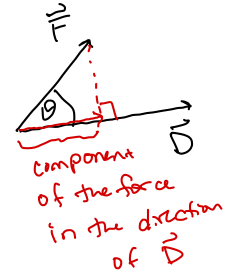
\includegraphics[height=1.5in]{Ch10s3-work2.png}
\caption{Diagram illustrating a Force vector projected onto a Displacement vector.}
\end{figure}
%\vspace*{1in}
%
%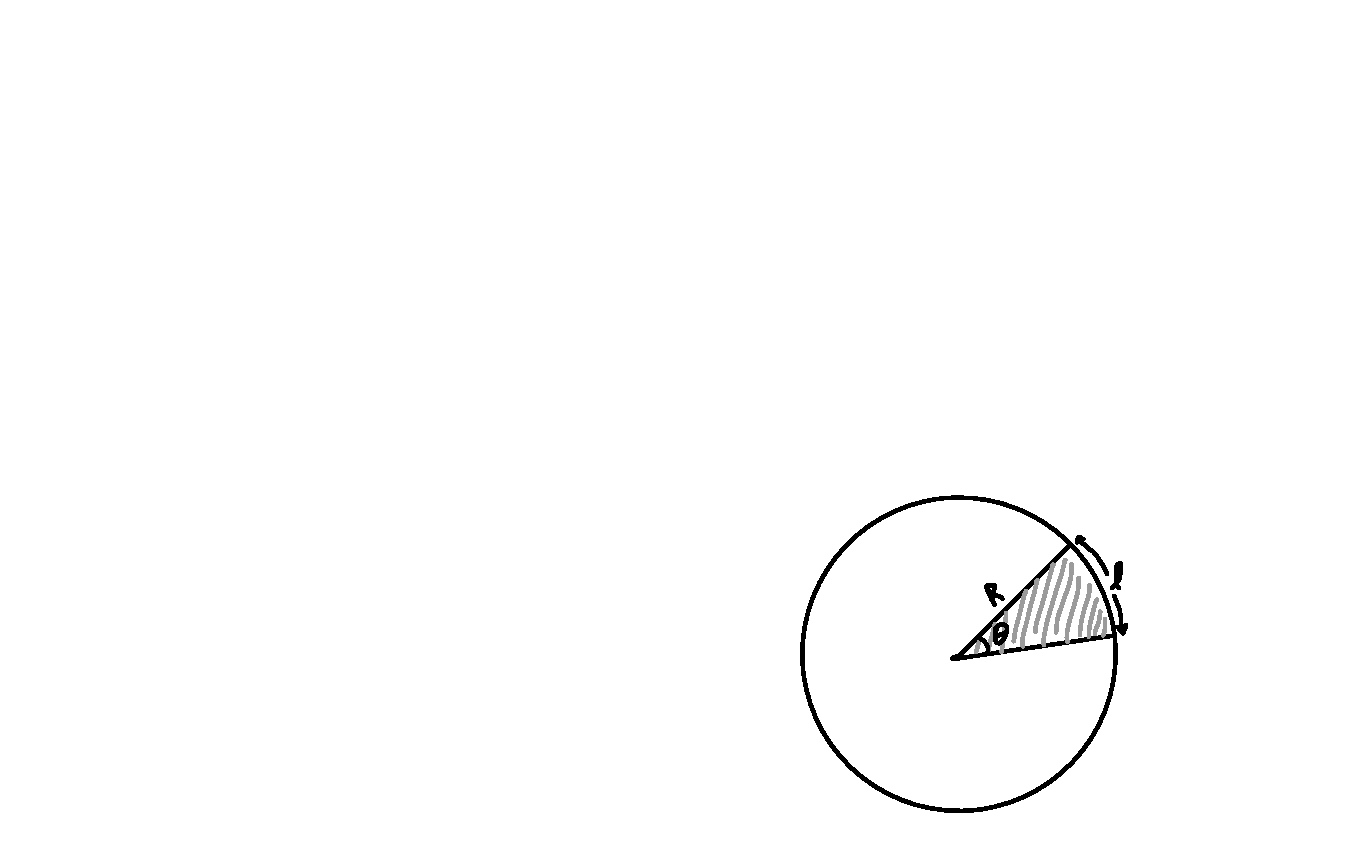
\includegraphics[height=1.5in]{circular-sector}


%\end{minipage}
\hspace*{.2in}
%\begin{minipage}{.5\textwidth}

The \textbf{work} done by a force \(\vec{F}\) to move an object a distance \(|\vec{D}|\) is calculated using:

\[W = \vec{F}\cdot \vec{D} = ||\vec{F}||\ ||\vec{D}||\ \cos \theta\]

\vspace*{.5in}

%\end{minipage}


%\end{framed}
%\end{minipage}

\textbf{Example 1:}
Show that the standard basis vectors are mutually orthogonal.

\vfill

\textbf{Example 2:}\\
Suppose a constant force of magnitude 50 lbs. acts on a sled that is being pulled through the snow a distance of 20 ft, and the force is applied at an angle \(\theta\) above the horizontal. How much work is done is \(\theta = \pi/3\)? \(\theta = \pi/4\)?

\vfill

\pagebreak

\section*{Group Work:}

\begin{center}
\textbf{\Large The Regular Hexagon}\\
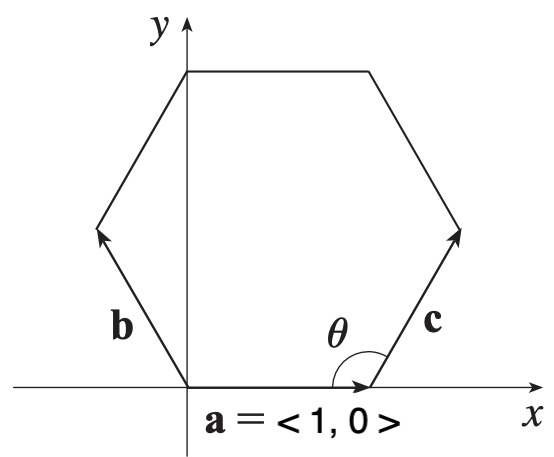
\includegraphics[width=.3\textwidth]{Ch2s3-hexagon2.png}
%\vspace*{-2in}
\end{center}
Consider the regular hexagon shown above.

\begin{enumerate}

\item Compute \(||\a||, ||\b||, \text{ and } ||\c||\).

\vfill

\item What is the angle labeled \(\theta\)\ ?

\vfill

\item What is \(\a \cdot \c\)\ ?

\vfill

\item What is \(\a \cdot \b\)\ ?

\vfill

\item What are \(\text{proj}_{\a} \c\) and \(\text{proj}_{\b} \c\)\ ?

\vfill

\item What is the \(x-\)component of \(\a+\b+\c\)\ ?

\vfill


\end{enumerate}

\end{document}
